\section{Git Branches}
\begin{frame}[fragile]
  \slidetitle

  This section covers the following topics:
  \begin{itemize}
    \item Create and delete branches
    \item Work with branches
    \item Rebase branches
    \item Merge branches
    \item Cherry-Pick commits
  \end{itemize}
\end{frame}

\subsection{The master branch}
\begin{frame}[fragile]
  \subslidetitle

  With git, you are always working on a branch and the default git branch is called \cmd{master}.
  \newline \vspace{1em}
  \centerline{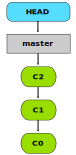
\includegraphics{assets/diagrams/branch-master.pdf}}

  \vspace{1.2em}
  Note: \cmd{HEAD} always points to the current branch.

\end{frame}

\subsection{Creating branches}
\begin{frame}[fragile]
  \subslidetitle

  To create a new \cmd{foo} branch, append the branch name to the \cmd{git branch} command:
  \begin{lstlisting}
(*\textcolor[HTML]{18B2B2}{(master)}*) $ (*\textcolor[HTML]{0000AA}{git branch foo}*)
\end{lstlisting}

  The \cmd{git branch} command lists all your local branches:
  \begin{lstlisting}
(*\textcolor[HTML]{18B2B2}{(master)}*) $ (*\textcolor[HTML]{0000AA}{git branch}*)
  foo
* (*\textcolor[HTML]{00AA00}{master}*)
\end{lstlisting}
  \vspace{1em}
  \centerline{
\includegraphics{assets/diagrams/branch-create.pdf}}
  \vspace{1em}
  Note: The branch you are currently on is marked with an asterisk (*).
\end{frame}

\subsection{Switching to branch}
\begin{frame}[fragile]
  \subslidetitle
  The \cmd{git switch} command is used to change the current branch:
  \begin{lstlisting}
(*\textcolor[HTML]{18B2B2}{(master)}*) $ (*\textcolor[HTML]{0000AA}{git switch foo}*)
Switched to branch 'foo'

(*\textcolor[HTML]{18B2B2}{(foo)}*) $ (*\textcolor[HTML]{0000AA}{git branch}*)
* (*\textcolor[HTML]{00AA00}{foo}*)
  master
\end{lstlisting}

  \vspace{1em}
  The \cmd{git switch} command with \cmd{-c} option creates a new branch and automatically switches to it:
  \begin{lstlisting}
(*\textcolor[HTML]{18B2B2}{(foo)}*) $ (*\textcolor[HTML]{0000AA}{git switch -c bar}*)
Switched to a new branch 'bar'

(*\textcolor[HTML]{18B2B2}{(bar)}*) $ (*\textcolor[HTML]{0000AA}{git branch}*)
* (*\textcolor[HTML]{00AA00}{bar}*)
  foo
  master
\end{lstlisting}
\end{frame}

\subsection{Deleting a branch}
\begin{frame}[fragile]
  \subslidetitle
  To delete an existing branch use the \cmd{-d} or \cmd{-D} (force) flag:
\begin{lstlisting}
(*\textcolor[HTML]{18B2B2}{(bar)}*) $ (*\textcolor[HTML]{0000AA}{git switch master}*)

(*\textcolor[HTML]{18B2B2}{(master)}*) $ (*\textcolor[HTML]{0000AA}{git branch -d foo bar}*)
Deleted branch foo (was c974445).
Deleted branch bar (was 9adadac).

(*\textcolor[HTML]{18B2B2}{(master)}*) $ (*\textcolor[HTML]{0000AA}{git branch}*)
* (*\textcolor[HTML]{00AA00}{master}*)
\end{lstlisting}

  \vspace{1em}
  Note: you cannot delete the branch you are currently working on.
\end{frame}

\subsection{Rebasing}
\begin{frame}[fragile]
  \subslidetitle
  Rebase puts a branch on top of an other:
  \centerline{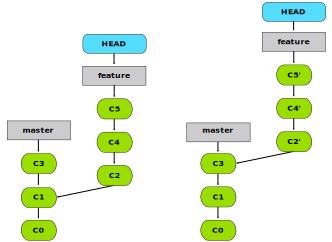
\includegraphics{assets/diagrams/branch-rebase.pdf}}
\end{frame}

\subsection{Prepare for rebase exercise}
\begin{frame}[fragile]
  \subslidetitle

  Start to create a new fix-title branch:
  \begin{lstlisting}
(*\textcolor[HTML]{18B2B2}{(master)}*) $ (*\textcolor[HTML]{0000AA}{git switch -c fix-title}*)
Switched to a new branch 'fix-title'
\end{lstlisting}

  Modify the \cmd{moon.html} according to this diff instructions:
  \begin{lstlisting}
(*\textcolor[HTML]{18B2B2}{@@ -7,7 +7,8 @@}*)
        font-family: Monospace;
(*\textcolor[HTML]{AA0000}{-}*)        (*\textcolor[HTML]{AA0000}{background-color: \#f0f0f0; <!-- grey -->}*)
(*\textcolor[HTML]{AA0000}{-}*)        (*\textcolor[HTML]{AA0000}{color: black;}*)
(*\textcolor[HTML]{00AA00}{+}*)        (*\textcolor[HTML]{00AA00}{background-color: black;}*)
(*\textcolor[HTML]{00AA00}{+}*)        (*\textcolor[HTML]{00AA00}{color: white;}*)
        margin: 0px;
\end{lstlisting}
\end{frame}

\subsection{Prepare for rebase exercise}
\begin{frame}[fragile]
  \subslidetitle
  Staging of all modification can be done with \cmd{-a}:
  \begin{lstlisting}
(*\textcolor[HTML]{18B2B2}{(fix-title)}*) $ (*\textcolor[HTML]{0000AA}{git commit -a -m "change title background color"}*)
[fix-title 95cb48c] change title background color
 1 file changed, 2 insertions(+), 2 deletions(-)
\end{lstlisting}

\end{frame}

\subsection{Display difference between branches}
\begin{frame}[fragile]
  \subslidetitle

  As git has the complete history locally, we can easily display changes between branches:

  \begin{lstlisting}
(*\textcolor[HTML]{18B2B2}{(fix-title)}*) $ (*\textcolor[HTML]{0000AA}{git diff master}*)
diff --git a/moon.html b/moon.html
index 145cfff..ae7bc15 100644
--- a/moon.html
+++ b/moon.html
(*\textcolor[HTML]{18B2B2}{@@ -7,7 +7,8 @@}*)
   <style>
     body {
         font-family: Monospace;
(*\textcolor[HTML]{AA0000}{-}*)         (*\textcolor[HTML]{AA0000}{background-color: \#f0f0f0; <!-- grey -->}*)
(*\textcolor[HTML]{AA0000}{-}*)         (*\textcolor[HTML]{AA0000}{color: black;}*)
(*\textcolor[HTML]{00AA00}{+}*)         (*\textcolor[HTML]{00AA00}{background-color: black;}*)
(*\textcolor[HTML]{00AA00}{+}*)         (*\textcolor[HTML]{00AA00}{color: white;}*)
         margin: 0px;
         overflow: hidden;
     }
\end{lstlisting}
\end{frame}

\subsection{Prepare for rebase exercise}
\begin{frame}[fragile]
  \subslidetitle

  In the meantime, we need to update the README.md file with a prerequisites sub-section:
  \begin{lstlisting}
(*\textcolor[HTML]{18B2B2}{(fix-title)}*) $ (*\textcolor[HTML]{0000AA}{git switch master}*)
Switched to branch 'master'
Your branch is ahead of 'origin/master' by 6 commits.
  (use "git push" to publish your local commits)

(*\textcolor[HTML]{18B2B2}{(master)}*) $ (*\textcolor[HTML]{0000AA}{echo "\#\# Prerequisites" >> README.md}*)

(*\textcolor[HTML]{18B2B2}{(master)}*) $ (*\textcolor[HTML]{0000AA}{git commit -a -m "document prerequisites"}*)
[master 3b8408d] document prerequisites
 1 file changed, 1 insertion(+)
\end{lstlisting}

  \centerline{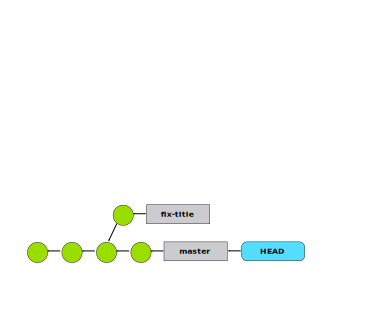
\includegraphics{assets/diagrams/rebase-situation-before.pdf}}

\end{frame}

\subsection{Rebasing a branch}
\begin{frame}[fragile]
  \subslidetitle

  Use \cmd{git rebase} to update the status of a branch on top of another branch:

  \begin{lstlisting}
(*\textcolor[HTML]{18B2B2}{(master)}*) $ (*\textcolor[HTML]{0000AA}{git switch fix-title}*)

(*\textcolor[HTML]{18B2B2}{(fix-title)}*) $ (*\textcolor[HTML]{0000AA}{git rebase master}*)
First, rewinding head to replay your work on top of it...
Applying: change title background color
\end{lstlisting}

  As git states the rebase re-applies commits from the fix-title branches on to of the master branch.

  \vspace{1em}
  \centerline{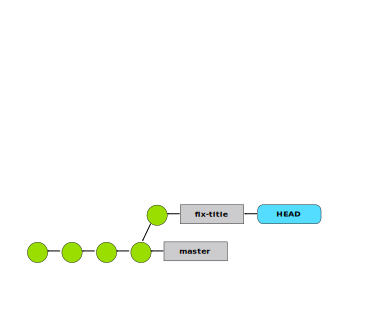
\includegraphics{assets/diagrams/rebase-situation-after.pdf}}

\end{frame}

\subsection{Merging}
\begin{frame}[fragile]
  \subslidetitle
  Merge integrates a branch into another:
  \centerline{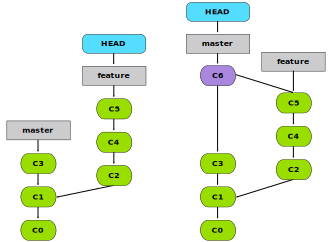
\includegraphics{assets/diagrams/branch-merge.pdf}}
\end{frame}

\subsection{Prepare for merge exercise}
\begin{frame}[fragile]
  \subslidetitle

  Let's create a new \cmd{third-moon} branch:
  \begin{lstlisting}
(*\textcolor[HTML]{18B2B2}{(fix-title)}*) $ (*\textcolor[HTML]{0000AA}{git switch -c third-moon master}*)
Switched to a new branch 'third-moon'
\end{lstlisting}

  Modify the \cmd{moon.js} file following this diff instructions:
  \begin{lstlisting}
(*\textcolor[HTML]{18B2B2}{@@ -3,6 +3,7 @@}*)

 // create moons
 new Moon("blue");
(*\textcolor[HTML]{00AA00}{+}*)(*\textcolor[HTML]{00AA00}{new Moon("white");}*)
 new Moon("green");
\end{lstlisting}
  Commit your changes:
  \begin{lstlisting}
(*\textcolor[HTML]{18B2B2}{(third-moon)}*) $ (*\textcolor[HTML]{0000AA}{git commit -a -m "add white moon in the middle"}*)
\end{lstlisting}
\end{frame}

\subsection{Prepare for merge exercise}
\begin{frame}[fragile]
  \subslidetitle

  Let's make a change on master branch:
  \begin{lstlisting}
(*\textcolor[HTML]{18B2B2}{(third-moon)}*) $ (*\textcolor[HTML]{0000AA}{git switch master}*)
Switched to branch 'master'
Your branch is ahead of 'origin/master' by 7 commits.
  (use "git push" to publish your local commits)
\end{lstlisting}

  Modify the README.md as following:
  \begin{lstlisting}
(*\textcolor[HTML]{18B2B2}{(master)}*) $ (*\textcolor[HTML]{0000AA}{echo " *\ Use a WebGL compatible browser" >> README.md}*)
\end{lstlisting}

  Commit your changes:
  \begin{lstlisting}
(*\textcolor[HTML]{18B2B2}{(master)}*) $ (*\textcolor[HTML]{0000AA}{git commit -a -m "doc: add prerequisites"}*)
[master 9c5f88d] doc: add prerequisites
 1 file changed, 1 insertion(+)
\end{lstlisting}

  \centerline{
\includegraphics{assets/diagrams/merge-situation-before.pdf}}

\end{frame}

\subsection{Merging a branch}
\begin{frame}[fragile]
  \subslidetitle

  Use \cmd{git merge} to merge a branch into another branch:

  \begin{lstlisting}
(*\textcolor[HTML]{18B2B2}{(master)}*) $ (*\textcolor[HTML]{0000AA}{git merge third-moon}*)
Merge branch 'third-moon' into master

# Please enter a commit message to explain why this merge is necessary,
# especially if it merges an updated upstream into a topic branch.
#
# Lines starting with '#' will be ignored, and an empty message aborts
# the commit.
\end{lstlisting}

  Save and exit the editor.
  \centerline{
\includegraphics{assets/diagrams/merge-situation-after.pdf}}

\end{frame}

\subsection{Cherry-Pick a commit}
\begin{frame}[fragile]
  \subslidetitle
  Instead of rebasing or merging entire branches, you can \textit{pick} single commits. \\

  Let's setup a branch and add two commits to setup the situation. \\
  \vspace{1em}
  The first commit should remove the blue moon form \cmd{moon.js}: \\
  \begin{lstlisting}
(*\textcolor[HTML]{18B2B2}{(master)}*) $ (*\textcolor[HTML]{0000AA}{git switch -c no-blue}*)
(*\textcolor[HTML]{18B2B2}{(no-blue)}*) $ (*\textcolor[HTML]{0000AA}{git commit -a -m "remove the blue moon"}*)
\end{lstlisting}

  The second commit should change the \cmd{README.md}:\\
  \begin{lstlisting}
(*\textcolor[HTML]{18B2B2}{(no-blue)}*) $ (*\textcolor[HTML]{0000AA}{echo " *\ Use a good screen" >> README.md}*)
(*\textcolor[HTML]{18B2B2}{(no-blue)}*) $ (*\textcolor[HTML]{0000AA}{git commit -a -m "note screen prerequisites"}*)
\end{lstlisting}
  \vspace{1em}
  \centerline{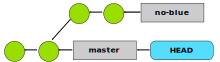
\includegraphics{assets/diagrams/cherry-pick-before.pdf}}
\end{frame}

\subsection{Cherry-Pick a commit}
\begin{frame}[fragile]
  \subslidetitle
    Now we want to switch back to master and only apply the \lstinline{1d36adc - remove the blue moon} commit.
    Thus, let's use \cmd{git cherry-pick}:
  \begin{lstlisting}
(*\textcolor[HTML]{18B2B2}{(no-blue)}*) $ (*\textcolor[HTML]{0000AA}{git switch master}*)
Switched to branch 'master'
\end{lstlisting}

  Now we \textit{cherry-pick} the preceding commit:
  \begin{lstlisting}
(*\textcolor[HTML]{18B2B2}{(master)}*) $ (*\textcolor[HTML]{0000AA}{git cherry-pick 1d36adc}*)
[master fbd4ca8] remove the blue moon
 Date: Sun Nov 29 10:06:27 2015 +0000
 1 file changed, 1 deletion(-)
\end{lstlisting}

  \vspace{1em}

  \centerline{
\includegraphics{assets/diagrams/cherry-pick-after.pdf}}
\end{frame}

\subsection{Stashing modifications}
\begin{frame}[fragile]
  \subslidetitle

  Edit the README.md file:
  \begin{lstlisting}
(*\textcolor[HTML]{18B2B2}{(master)}*)$ (*\textcolor[HTML]{0000AA}{echo " *\ openGl drivers installed" >> README.md}
\end{lstlisting}

  Imagine you are in the middle of a modification.

  \begin{lstlisting}
(*\textcolor[HTML]{18B2B2}{(master)}*)$ (*\textcolor[HTML]{0000AA}{git status}*)
...
       (*\textcolor[HTML]{AA0000}{modified:   README.md}*)
...
\end{lstlisting}

  \vspace{2em}
  And suddenly something really important needs to be done immediately on the fix-title branch! 

  \begin{lstlisting}
(*\textcolor[HTML]{18B2B2}{(master)}*)$ (*\textcolor[HTML]{0000AA}{git switch fix-title}*)
\end{lstlisting}
\end{frame}

\subsection{Stashing modifications}
\begin{frame}[fragile]
  \subslidetitle

  \begin{lstlisting}
(*\textcolor[HTML]{18B2B2}{(master)}*)$ (*\textcolor[HTML]{0000AA}{git stash}*)
Saved working directory and index state WIP on master: 80c8cac Merge branch 'third-moon'
HEAD is now at 80c8cac Merge branch 'third-moon'
(*\textcolor[HTML]{18B2B2}{(master)}*)$ (*\textcolor[HTML]{0000AA}{git status}*)
On branch master
...
nothing to commit (working directory clean)
\end{lstlisting}
  Note: you now have a clean working directory again.
\end{frame}

\subsection{Display stash stack}
\begin{frame}[fragile]
  \subslidetitle
  Do not worry, \cmd{git stash} does not loose any information, let's have a look:

  \begin{lstlisting}
(*\textcolor[HTML]{18B2B2}{(master)}*)$ (*\textcolor[HTML]{0000AA}{git stash list}*)
stash@{0}: WIP on master: 80c8cac Merge branch 'third-moon'
(END)
\end{lstlisting}
  Show what was stashed with \cmd{git stash show}:
  \begin{lstlisting}
(*\textcolor[HTML]{18B2B2}{(master)}*)$ (*\textcolor[HTML]{0000AA}{git stash show stash@\{0\}}*)
README.md | 1 +
 1 file changed, 1 insertion(+)
(END)
\end{lstlisting}

\end{frame}

\subsection{Restore stashed changes}
\begin{frame}[fragile]
  \subslidetitle

  \begin{lstlisting}
(*\textcolor[HTML]{18B2B2}{(master)}*)$ (*\textcolor[HTML]{0000AA}{git stash pop}*)
On branch master
Changes not staged for commit:
   (use "git add <file>..." to update what will be committed)
   (use "git restore <file>..." to discard changes in working directory)
       (*\textcolor[HTML]{AA0000}{modified:}*)   (*\textcolor[HTML]{AA0000}{README.md}*)
no changes added to commit (use "git add" and/or "git commit -a")
Dropped refs/stash@{0} (ac514d6d83880d45ca994d4b83b485340f192a7e)
\end{lstlisting}
  Discard the previous changes:
  \begin{lstlisting}
(*\textcolor[HTML]{18B2B2}{(master)}*)$ (*\textcolor[HTML]{0000AA}{git restore README.md}*)
\end{lstlisting}
\end{frame}

\subsection{Summary}
\begin{frame}[fragile]
\subslidetitle
  What we've learned in this chapter:
  \begin{itemize}
    \item Create and delete branches
    \item Switch branches
    \item Rebase branches
    \item Merge branches
    \item Cherry-pick commits
    \item Working with stashes
  \end{itemize}
\end{frame}
